\section{Konversi NFA ke DFA: Subset Construction}

Karena NFA tidak deterministik dan simulasi NFA bisa tidak efisien, kita perlu mengkonversi NFA menjadi DFA yang ekuivalen menggunakan algoritma \textbf{subset construction}.

\subsection{Konsep \texorpdfstring{$\epsilon$}{epsilon}-Closure}

Sebelum subset construction, kita perlu memahami konsep \textbf{$\epsilon$-closure}:

\begin{itemize}
    \item \textbf{$\epsilon$-closure} dari suatu state adalah himpunan semua state yang dapat dicapai dari state tersebut melalui $\epsilon$-transitions saja
    \item \textbf{$\epsilon$-closure} dari suatu set states adalah union dari $\epsilon$-closure setiap state dalam set tersebut
\end{itemize}

\subsection{Algoritma Subset Construction}

Algoritma subset construction bekerja sebagai berikut:

\begin{enumerate}
    \item \textbf{Start State DFA}: $\epsilon$-closure dari start state NFA
    \item \textbf{Untuk setiap state DFA dan setiap input symbol}:
    \begin{enumerate}
        \item Hitung semua NFA states yang dapat dicapai dengan input symbol tersebut
        \item Ambil $\epsilon$-closure dari set states tersebut
        \item Jika hasilnya belum ada sebagai state DFA, buat state baru
        \item Tambahkan transisi dari state DFA saat ini ke state hasil
    \end{enumerate}
    \item \textbf{Accept States DFA}: Setiap state DFA yang mengandung accept state NFA
\end{enumerate}

\subsection{Contoh: Konversi NFA \texttt{(a|b)*abb} ke DFA}

Mari kita ikuti langkah-langkah subset construction. Gambar \ref{fig:subset-construction} menunjukkan proses konversi dan hasil DFA yang dihasilkan.

\begin{enumerate}
    \item \textbf{Start State DFA}: 
    \begin{itemize}
        \item Mulai dari start state NFA, ambil $\epsilon$-closure
        \item Misalkan hasilnya adalah set $\{q_0, q_1, q_4\}$ → ini menjadi state DFA $A$
    \end{itemize}
    
    \item \textbf{Transisi dari State A dengan input 'a'}:
    \begin{itemize}
        \item Dari semua NFA states dalam A, cari yang dapat menerima 'a'
        \item Ambil $\epsilon$-closure dari hasilnya → misalkan $\{q_2, q_4, q_5\}$ → state DFA $B$
    \end{itemize}
    
    \item \textbf{Transisi dari State A dengan input 'b'}:
    \begin{itemize}
        \item Dari semua NFA states dalam A, cari yang dapat menerima 'b'
        \item Ambil $\epsilon$-closure dari hasilnya → misalkan $\{q_3, q_4\}$ → state DFA $C$
    \end{itemize}
    
    \item \textbf{Lanjutkan untuk state B dan C} dengan cara yang sama
    \item \textbf{Accept States}: State DFA yang mengandung accept state NFA (misalnya state yang mengandung $q_7$)
\end{enumerate}

\begin{figure}[!htbp]
    \centering
    \adjustbox{max width=0.85\textwidth,center}{%
    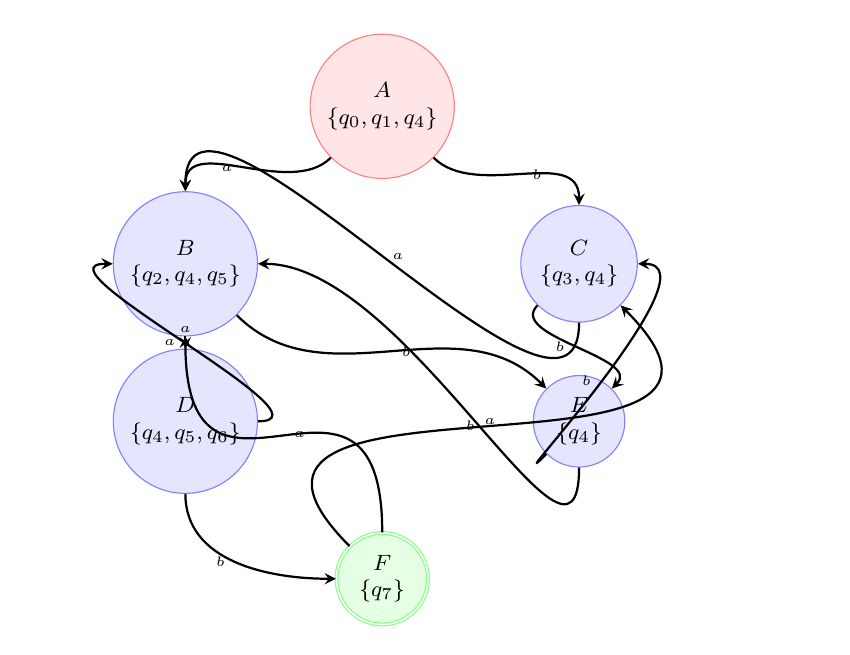
\begin{tikzpicture}[
        state/.style={circle, draw=blue!50, fill=blue!10, minimum size=0.7cm, font=\footnotesize, align=center},
        accept/.style={circle, draw=green!50, fill=green!10, minimum size=0.7cm, font=\footnotesize, double, align=center},
        start/.style={circle, draw=red!50, fill=red!10, minimum size=0.7cm, font=\footnotesize, align=center},
        arrow/.style={->, >=stealth, thick},
        node distance=2.5cm and 2cm
    ]
    
    % DFA States
    \node[start] (A) at (0,0) {$A$\\$\{q_0,q_1,q_4\}$};
    \node[state] (B) at (-2.5,-2) {$B$\\$\{q_2,q_4,q_5\}$};
    \node[state] (C) at (2.5,-2) {$C$\\$\{q_3,q_4\}$};
    \node[state] (D) at (-2.5,-4) {$D$\\$\{q_4,q_5,q_6\}$};
    \node[state] (E) at (2.5,-4) {$E$\\$\{q_4\}$};
    \node[accept] (F) at (0,-6) {$F$\\$\{q_7\}$};
    
    % Transitions
    \draw[arrow] (A) to[out=225, in=90] node[left, font=\tiny] {$a$} (B);
    \draw[arrow] (A) to[out=315, in=90] node[right, font=\tiny] {$b$} (C);
    \draw[arrow] (B) to[out=270, in=90] node[left, font=\tiny] {$a$} (D);
    \draw[arrow] (B) to[out=315, in=135] node[right, font=\tiny] {$b$} (E);
    \draw[arrow] (C) to[out=270, in=90] node[right, font=\tiny] {$a$} (B);
    \draw[arrow] (C) to[out=225, in=45] node[left, font=\tiny] {$b$} (E);
    \draw[arrow] (D) to[out=270, in=180] node[left, font=\tiny] {$b$} (F);
    \draw[arrow] (D) to[out=0, in=180] node[above, font=\tiny] {$a$} (B);
    \draw[arrow] (E) to[out=270, in=0] node[right, font=\tiny] {$a$} (B);
    \draw[arrow] (E) to[out=225, in=0] node[left, font=\tiny] {$b$} (C);
    \draw[arrow] (F) to[out=90, in=270, looseness=2] node[right, font=\tiny] {$a$} (B);
    \draw[arrow] (F) to[out=135, in=315, looseness=2] node[left, font=\tiny] {$b$} (C);
    
    \end{tikzpicture}%
    }
    \caption{DFA hasil subset construction dari NFA \texttt{(a|b)*abb}}
    \label{fig:subset-construction}
\end{figure}

Hasilnya adalah DFA yang ekuivalen dengan NFA asli, tetapi deterministik dan lebih efisien untuk simulasi. Setiap state DFA merepresentasikan set states NFA yang dapat dicapai dengan input tertentu.